\section{Analysis}
\label{sec:Analysis}
This section gives some tips to analyze a COMPSs trace from two different points of view:
graphically and numerically.

\subsection{Graphical Analysis}
The main concept is that computational events, the task events in this case, must be well 
distributed among all workers to have a good parallelism, and the duration of task events 
should be also balanced, this means, the duration of computational bursts.

\begin{figure}[ht!]
  \centering
    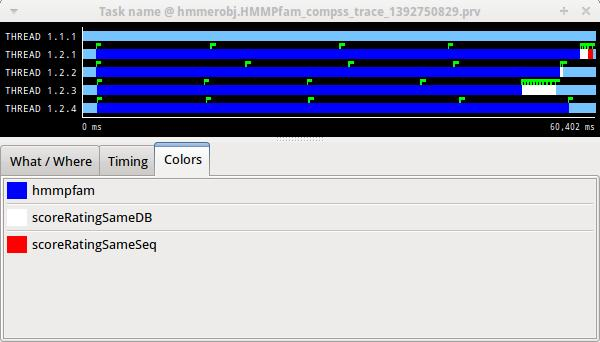
\includegraphics[width=1.0\textwidth]{./Sections/5_Analysis/Figures/8.jpeg}
    \caption{Basic trace view of a Hmmpfam execution.}
\end{figure}

In the previous trace view, all the tasks of type ``hmmpfam'' in dark blue appear to be well 
distributed among the four workers, each worker executes four ``hmmpfam'' tasks.

However, some workers finish earlier than the others, worker 1.2.3 finish the first and worker 1.2.1 
the last. So there is an imbalance in the duration of ``hmmpfam'' tasks. The programmer should 
analyze then whether all the tasks process the same amount of input data and do the same thing 
in order to find out the reason for such imbalance.

Another thing to highlight is that tasks of type ``scoreRatingSameDB'' are not equally distributed 
among all the workers. Some workers execute more tasks of this type than the others. 
To understand better what happens here, one needs to take a look to the execution graph and also zoom 
in the last part of the trace.

\begin{figure}[ht!]
  \centering
    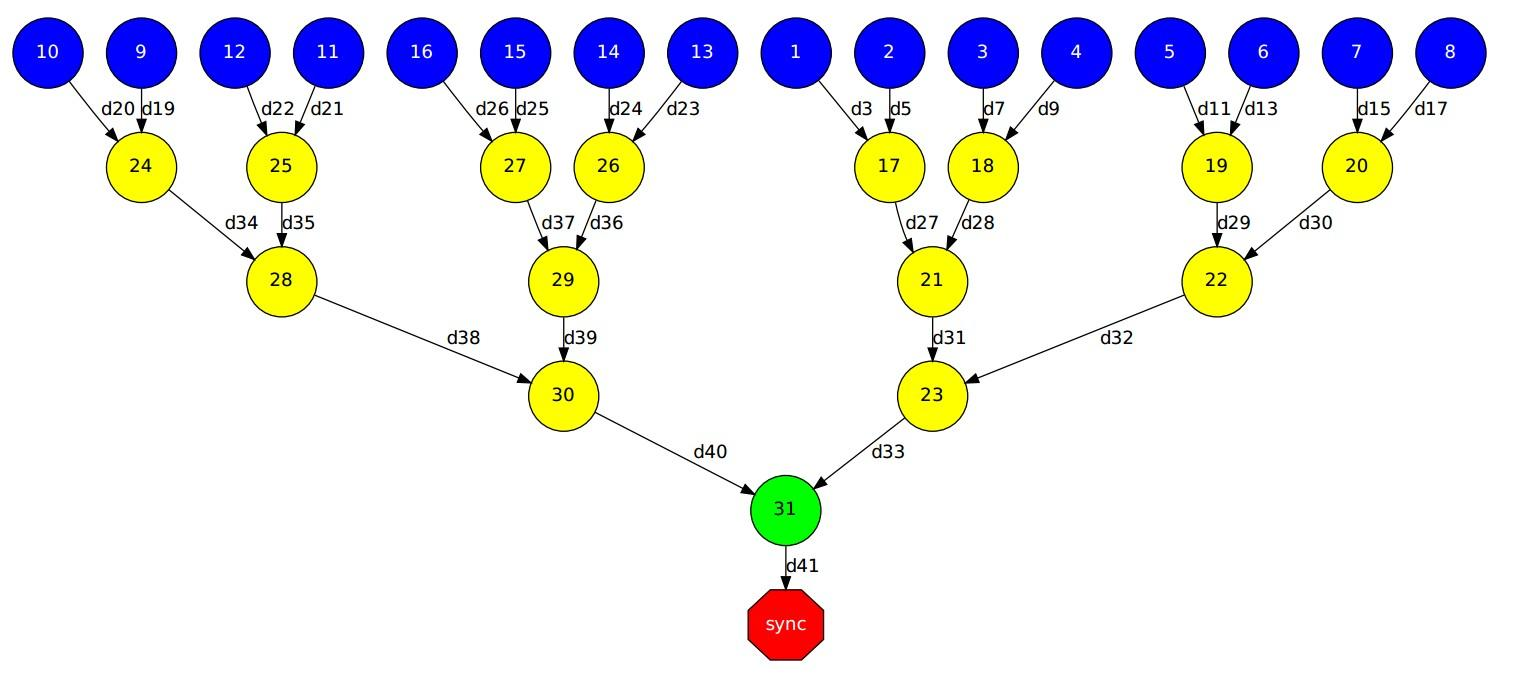
\includegraphics[width=1.0\textwidth]{./Sections/5_Analysis/Figures/9.jpeg}
    \caption{Data dependencies graph of a Hmmpfam execution.}
\end{figure}

\begin{figure}[ht!]
  \centering
    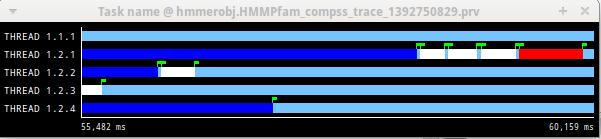
\includegraphics[width=1.0\textwidth]{./Sections/5_Analysis/Figures/10.jpeg}
    \caption{Zoomed in view of a Hmmpfam execution.}
\end{figure}

There is only one task of type ``scoreRatingSameSeq''. This task appears in red in the trace 
(and in light-green in the graph). With the help of the graph we see that the ``scoreRatingSameSeq'' 
task has dependences on tasks of type ``scoreRatingSameDB'', in white (or yellow).

When the last task of type ``hmmpfam'' (in dark blue) ends, the previous dependencies are solved, 
and if we look at the graph, this means going across a path of three dependencies of type 
``scoreRatingSameDB'' (in yellow). Moreover, because these are sequential dependencies (one depends 
on the previous) no more than a worker can be used at the same time to execute the tasks. 
This is the reason of why the last three task of type ``scoreRatingSameDB'' (in white) are 
executed in worker 1.2.1 sequentially.

\subsection{Numerical Analysis}
Here we show another trace from a different parallel execution of the Hmmer program.
 
\begin{figure}[ht!]
  \centering
    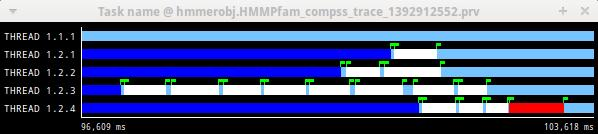
\includegraphics[width=1.0\textwidth]{./Sections/5_Analysis/Figures/11.jpeg}
    \caption{Original sample trace interval corresponding to the obtained Histogram.}
\end{figure} 
 
Paraver offers the possibility of having different histograms of the trace events. 
Click the ``New Histogram'' button in the main window and accept the 
default options in the ``New Histogram'' window that will appear.

\begin{figure}[ht!]
  \centering
    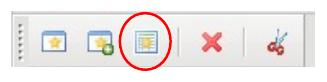
\includegraphics[width=0.5\textwidth]{./Sections/5_Analysis/Figures/12.jpeg}
    \caption{Paraver Menu - New Histogram}
\end{figure}

After that, the following table is shown. In this case for each worker, the time spent 
executing each type of task is shown. Task names appear in the same color than in the 
trace view. The color of a cell in a row corresponding to a worker ranges from 
light-green for lower values to dark-blue for higher ones. This conforms a color based histogram.

\begin{figure}[ht!]
  \centering
    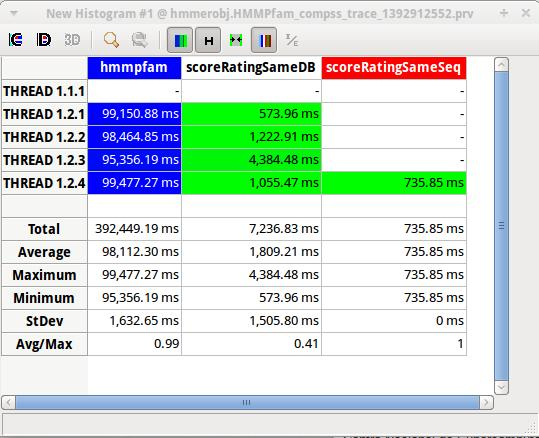
\includegraphics[width=0.8\textwidth]{./Sections/5_Analysis/Figures/13.jpeg}
    \caption{Hmmpfam histogram corresponding to previous trace}
\end{figure}
 
The previous table also gives, at the end of each column, some extra statistical 
information for each type of tasks (as the total, average, maximum or minimum values, etc.).

\newpage
In the window properties of the main window, it is possible to change the semantic of the statistics 
to see other factors rather than the time, for example, the number of bursts.

\begin{figure}[ht!]
  \centering
    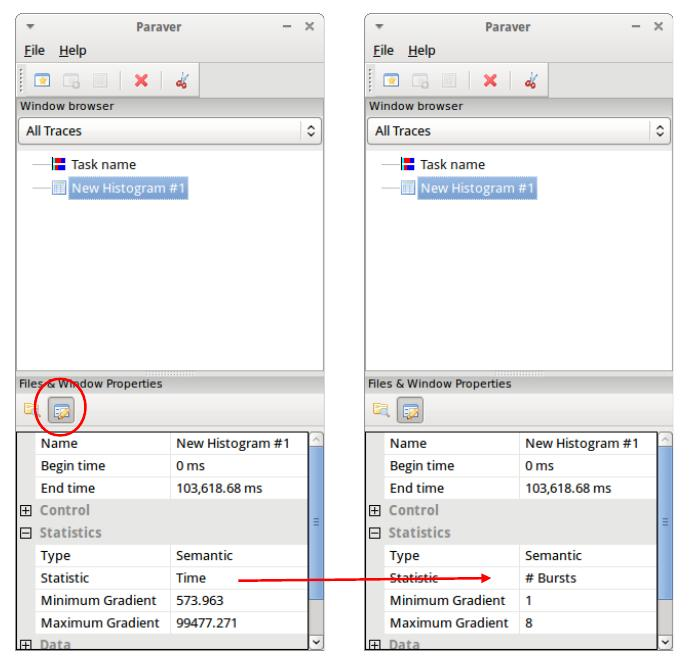
\includegraphics[width=0.8\textwidth]{./Sections/5_Analysis/Figures/14.jpeg}
    \caption{Paraver histogram options menu}
\end{figure}

\newpage
In the same way as before, the following table shows for each worker the number of bursts 
for each type of task, this is, the number or tasks executed of each type. Notice the gradient 
scale from light-green to dark-blue changes with the new values.

\begin{figure}[ht!]
  \centering
    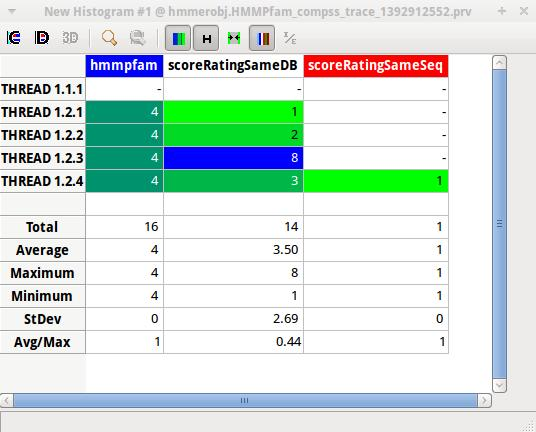
\includegraphics[width=0.8\textwidth]{./Sections/5_Analysis/Figures/15.jpeg}
    \caption{Hmmpfam histogram with the number of bursts}
\end{figure}